%me=0 student solutions (ps file), me=1 - my solutions (sol file), me=2 - assignment (hw file)
\def\me{0}
\def\num{7}  %homework number
\def\due{Tuesday, November 10}  %due date
\def\course{CSCI-GA.1170-001/002 Fundamental Algorithms} %course name, changed only once
\def\name{GOWTHAM GOLI (N17656180)}   %student changes (instructor keeps!)
%
\iffalse
INSTRUCTIONS: replace # by the homework number.
(if this is not ps#.tex, use the right file name)

  Clip out the ********* INSERT HERE ********* bits below and insert
appropriate TeX code.  Once you are done with your file, run

  ``latex ps#.tex''

from a UNIX prompt.  If your LaTeX code is clean, the latex will exit
back to a prompt.  To see intermediate results, type

  ``xdvi ps#.dvi'' (from UNIX prompt)
  ``yap ps#.dvi'' (if using MikTex in Windows)

after compilation. Once you are done, run

  ``dvips ps#.dvi''

which should print your file to the nearest printer.  There will be
residual files called ps#.log, ps#.aux, and ps#.dvi.  All these can be
deleted, but do not delete ps1.tex. To generate postscript file ps#.ps,
run

  ``dvips -o ps#.ps ps#.dvi''

I assume you know how to print .ps files (``lpr -Pprinter ps#.ps'')
\fi
%
\documentclass[11pt]{article}
\usepackage{amsfonts}
\usepackage{latexsym}
\usepackage[lined,boxed,linesnumbered]{algorithm2e}
\usepackage{amsmath}
\usepackage{amsthm}
\usepackage{array}
\usepackage{amssymb}
\usepackage{amsthm}
\usepackage{epsfig}
\usepackage{psfrag}
\usepackage{color}
\usepackage{tikz}
\usepackage{enumerate}
\usetikzlibrary{calc,trees,positioning,arrows,fit,shapes,calc}
\usetikzlibrary{trees}
\usepackage{mathtools}
\usepackage{float}
\setlength{\oddsidemargin}{.0in}
\setlength{\evensidemargin}{.0in}
\setlength{\textwidth}{6.5in}
\setlength{\topmargin}{-0.4in}
\setlength{\textheight}{8.5in}

\newcommand{\handout}[5]{
   \renewcommand{\thepage}{#1, Page \arabic{page}}
   \noindent
   \begin{center}
   \framebox{
      \vbox{
    \hbox to 5.78in { {\bf \course} \hfill #2 }
       \vspace{4mm}
       \hbox to 5.78in { {\Large \hfill #5  \hfill} }
       \vspace{2mm}
       \hbox to 5.78in { {\it #3 \hfill #4} }
      }
   }
   \end{center}
   \vspace*{4mm}
}

\newcounter{pppp}
\newcommand{\prob}{\arabic{pppp}}  %problem number
\newcommand{\increase}{\addtocounter{pppp}{1}}  %problem number

%first argument desription, second number of points
\newcommand{\newproblem}[2]{
\ifnum\me=0
\ifnum\prob>0 \newpage \fi
\increase
\setcounter{page}{1}
\handout{\name, Homework \num, Problem \arabic{pppp}}{\today}{Name: \name}{Due:
\due}{Solutions to Problem \prob\ of Homework \num\ (#2)}
\else
\increase
\section*{Problem \num-\prob~(#1) \hfill {#2}}
\fi
}

%\newcommand{\newproblem}[2]{\increase
%\section*{Problem \num-\prob~(#1) \hfill {#2}}
%}

\def\squarebox#1{\hbox to #1{\hfill\vbox to #1{\vfill}}}
\def\qed{\hspace*{\fill}
        \vbox{\hrule\hbox{\vrule\squarebox{.667em}\vrule}\hrule}}
\newenvironment{solution}{\begin{trivlist}\item[]{\bf Solution:}}
                      {\qed \end{trivlist}}
\newenvironment{solsketch}{\begin{trivlist}\item[]{\bf Solution Sketch:}}
                      {\qed \end{trivlist}}
\newenvironment{code}{\begin{tabbing}
12345\=12345\=12345\=12345\=12345\=12345\=12345\=12345\= \kill }
{\end{tabbing}}

%%%%%\newcommand{\eqref}[1]{Equation~(\ref{eq:#1})}

\newcommand{\hint}[1]{({\bf Hint}: {#1})}
%Put more macros here, as needed.
\newcommand{\room}{\medskip\ni}
\newcommand{\brak}[1]{\langle #1 \rangle}
\newcommand{\bit}[1]{\{0,1\}^{#1}}
\newcommand{\zo}{\{0,1\}}
\newcommand{\C}{{\cal C}}

\newcommand{\nin}{\not\in}
\newcommand{\set}[1]{\{#1\}}
\renewcommand{\ni}{\noindent}
\renewcommand{\gets}{\leftarrow}
\renewcommand{\to}{\rightarrow}
\newcommand{\assign}{:=}
\newcommand{\cT}{\mathcal{T}}

\newcommand{\AND}{\wedge}
\newcommand{\OR}{\vee}

\newcommand{\Forr}{\mbox{\bf For }}
\newcommand{\To}{\mbox{\bf to }}
\newcommand{\Do}{\mbox{\bf Do }}
\newcommand{\Ifi}{\mbox{\bf If }}
\newcommand{\Then}{\mbox{\bf Then }}
\newcommand{\Elsee}{\mbox{\bf Else }}
\newcommand{\Whilee}{\mbox{\bf While }}
\newcommand{\Repeatt}{\mbox{\bf Repeat }}
\newcommand{\Until}{\mbox{\bf Until }}
\newcommand{\Returnn}{\mbox{\bf Return }}
\newcommand{\Swap}{\mbox{\bf Swap }}

\begin{document}

\ifnum\me=0
%\handout{PS\num}{\today}{Name: **** INSERT YOU NAME HERE ****}{Due:
%\due}{Solutions to Problem Set \num}
%
%I collaborated with *********** INSERT COLLABORATORS HERE (INDICATING
%SPECIFIC PROBLEMS) *************.
\fi
\ifnum\me=1
\handout{PS\num}{\today}{Name: Yevgeniy Dodis}{Due: \due}{Solution
{\em Sketches} to Problem Set \num}
\fi
\ifnum\me=2
\handout{PS\num}{\today}{Lecturer: Yevgeniy Dodis}{Due: \due}{Problem
Set \num}
\fi

%1-2

\newproblem{Maximize Sum/Product}{14 points}



Suppose you are given an array $A[1, \ldots, n]$ of numbers, which may be positive, negative, or zero.

\begin{itemize}
\item[(a)] (4 points) Let $S_{i,j}$ denote $A[i] + A[i+1] + \cdots + A[j]$. Use dynamic programming to give an $O(n^2)$ algorithm to compute $S_{i, j}$ for all $1 \le i \le j \le n$, and hence compute $\max_{i, j} S_{i, j}$.
\ifnum\me<2
\begin{solution}
\[
S[i,j] = \begin{dcases*}
A[i] & if $i = j$\\
S[i,j-1]+A[j] & if  $i<j$
\end{dcases*}
\]

\IncMargin{1em}
\begin{algorithm*}[H]
\TitleOfAlgo{{\sc MaxSumSubArray}($A$)}
$S \leftarrow$ {\sc NewArray}($n \times n$)\\
$max \leftarrow -\infty$\\
\For{i $\leftarrow$ 1 to n}{
	$S[i,i] = A[i]$\\
	\uIf{S[i,i] $>$ max}{
		$max \leftarrow S[i,i]$\\
		$max_i \leftarrow i$, $max_j \leftarrow i$
	}
}
\For{i $\leftarrow$ 1 to n}{
	\For{j $\leftarrow$ i+1 to n}{
		$S[i,j] = S[i,j-1] + A[j]$\\
		\uIf{S[i,i] $>$ max}{
			$max \leftarrow S[i,j]$\\
			$max_i \leftarrow i$, $max_j \leftarrow j$
		}
	}
}
\Returnn ($max, max_i, max_j$)
\caption{Dynamic Programming Algorithm to calculate maximum sum sub-array in $O(n^2)$ time}
\end{algorithm*}

From the above two \textit{for} loops it is clear that the algorithm takes $O(n + n-1 + \ldots + 1) = O(n^2)$ time
\end{solution}
\fi

\item[(b)] (6 points) Let $L[j]$ denotes $\max_{i \le j} S_{i, j}$. Give a recurrence relation for $L[j]$ in terms of $L[1, \ldots, j-~1]$. Use your recurrence relation to give an $O(n)$ time dynamic programming algorithm to compute $L[1 \ldots n]$, and hence compute $\max_{i, j} S_{i,j}$.
\ifnum\me<2
\begin{solution}
\[
L[j] = \begin{dcases*}
A[1] & if $j=1$\\
A[j] & if $L[j-1] \leq 0$\\
L[j-1]+A[j] & if  $L[j-1] > 0$
\end{dcases*}
\]

\IncMargin{1em}
\begin{algorithm*}[H]
\TitleOfAlgo{{\sc MaxSumSubArray}($A$)}
$L \leftarrow$ {\sc NewArray}($n$)\\
$L[1] \leftarrow A[1]$\\
$max \leftarrow L[1]$\\
\For{i $\leftarrow$ 2 to n}{
	\uIf{L[i-1] $\leq$ 0}{
		$L[i] = A[i]$
	}
	\uElse{
		$L[i] = L[i-1] + A[i]$
	}
	\uIf{L[i] $>$ max}{
		$max \leftarrow L[i]$\\
	}
}
\Returnn $max$
\caption{Dynamic Programming Algorithm to calculate maximum sum sub-array in $O(n)$ time}
\end{algorithm*}
In the above algorithm, there is only one \textit{for} loop that runs from 2 to $n$. Hence the running time is $O(n)$
\end{solution}
\fi

\item[(c)] (2 points) Assume you use recursion (without memorization) to compute the answers to part(a) and part(b). Will both running times stay at $O(n^2)$ and $O(n)$, respectively, only one of them (which one?), or none?
\ifnum\me<2
\begin{solution}
\subsection*{Part(a)}
If we don't use the memory, then

Calculating the elements of the first row of the matrix takes $1+2+\ldots+n = O(n^2)$ time

Calculating the elements of the second row of the matrix takes $1+2+\ldots+n-1 = O((n-1)^2)$ time

$\vdots$

Calculating the elements of the last row of the matrix takes $1+2+\ldots+n-1 = O(1^2)$ time

Therefore, total time taken to calculate the matrix elements without memorization will be $O(1^2 + 2^2 + \ldots + (n-1)^2 + n^2) = O(n^3)$. The run time increases by a factor of $n$

\subsection*{Part(b)}

The running time will still be $O(n)$ without memorization using recursion. The maximum-sum-subarray of $A[1 \ldots j]$ makes a recursive call to maximum-sum-subarray of $A[1  \ldots j-1]$ which returns two fields, $L[j-1]$ which will be used to evaluate $L[j]$ and also the maximum sum sub array of $A[1 \ldots j-1]$. This maximum is compared to $L[j]$ and will be updated to $L[j]$ if it's lesser and return this maximum at the end. Thus the running time is sill $O(n)$ without using memorization 
\end{solution}
\fi
\pagebreak
\item[(d)] (4 points) Suggest appropriate modifications to your algorithm in part (b) to give an $O(n)$ algorithm to compute $\max_{i,j} P_{i,j}$, where
$P_{i,j} = A[i] \cdot A[i+1] \cdots A[j]$. Assume that multiplication of any two numbers takes $O(1)$ time.
\ifnum\me<2
\begin{solution}

Let $L[j]$ denotes $\max_{i \le j} P_{i, j}$, then

\[
L[j] = \begin{dcases*}
A[1] & if $j=1$\\
S[j-1]A[j] & if ($L[j-1] \leq 0$ and $A[j]  \leq 0$) or ($L[j-1] \geq 0$ and $A[j]  \geq 0$)\\
A[j] & if  ($L[j-1] > 0$ and $A[j] < 0$) or ($L[j-1] < 0$ and $A[j] > 0$)
\end{dcases*}
\]

\IncMargin{1em}
\begin{algorithm*}[H]
\TitleOfAlgo{{\sc MaxProductSubArray}($A$)}
$L \leftarrow$ {\sc NewArray}($n$)\\
$L[1] \leftarrow A[1]$\\
$max \leftarrow L[1]$\\
\For{j $\leftarrow$ 2 to n}{
	\uIf{($L[j-1] \leq 0$ and $A[j] \leq 0$) or ($L[j-1] \geq 0$ and $A[j]  \geq 0$)}{
		$L[j] = L[j-1]A[j]$
	}
	\uElseIf{($L[j-1] > 0$ and $A[j] < 0$) or ($L[j-1] < 0$ and $A[j] > 0$)}{
		$L[j] = A[j]$
	}
	\uIf{L[j] $>$ max}{
		$max \leftarrow L[j]$\\
	}
}
\Returnn $max$
\caption{Dynamic Programming Algorithm to calculate maximum product sub-array in $O(n)$ time}
\end{algorithm*}

Assuming that the multiplication of any two numbers takes $O(1)$ time, the running time of the above algorithm is clearly $O(n)$
\end{solution}
\fi
\end{itemize}


%1-11
\newproblem{Greatest Value Path}{8 points}

Assume that you have an $n$ by $n$ checkerboard. You must move a checker
from the bottom left corner (position $(1,1)$) square the board to the top right corner (position $(n,n)$)
square. In each step you may either
\begin{itemize}
\vspace{-1ex}
\item move the checker up one square, or
\vspace{-1ex}
\item move the checker diagonally one square up and to the right, or
\vspace{-1ex}
\item move the checker right one square.
\end{itemize}

If you move a checker from square $x=(i,j)$ to square $y=(i',j')$ you
get $p(x, y)$ dollars. You are told all of the $p(x, y)$ a priori. The
$p(x, y)$ may be negative, zero or positive. You want to get as much
money as possible.

\begin{itemize}
\item[(a)] (4 pts) Let $M[i,j]$ be the highest profit you can collect from position $(1,1)$ to $(i,j)$. Write a dynamic programming recurrence relation for $M[i,j]$ (do not forget the initial condition). Based on this recurrence relation, analyze the running time of the dynamic programming algorithm to compute $M[n,n]$.

\ifnum\me<2
\begin{solution}

The best way to get to any square $(i,j)$ is the best way to get from the square to it's left or the from the square to it's bottom or the from the diagonal square. Therefore,
\begin{align*}
M[i,j] = max\{& M[i,j-1]+p((i,j-1),(i,j)),\\& M[i-1,j-1]+p((i-1,j-1),(i,j)),\\& M[i-1,j] + p((i-1,j),(i,j))\}
\end{align*}

Note that the base case is $M[1,1] = 0$ and in the above equation, there will be no diagonal and bottom square for all the squares in the first row and there will be no diagonal and left squares for all the squares in the first column.

To fill an entry in the matrix $M$ we look the adjacent three entries and appropriately fill the corresponding entry. Therefore, the total time taken to build this matrix is $\leq 3n^2 = O(n^2)$


\end{solution}
\fi
\pagebreak
\item[(a)] (4 pts) Give the ``bottom-up" pseudocode for an efficient procedure {\sc CheckerBoard}$(n)$ for computing $M[n,n]$.

\ifnum\me<2
\begin{solution}

\IncMargin{1em}
\begin{algorithm*}[H]
\TitleOfAlgo{{\sc CheckerBoard}($n$)}
$M \leftarrow$ {\sc NewArray}($n \times n$)\\
$M[1,1] \leftarrow 0$\\
\For{i $\leftarrow$ 2 to n}{
	$M[i,1] \leftarrow M[i-1,1] + p((i-1,1),(i,1))$
}
\For{j $\leftarrow$ 2 to n}{
	$M[1,j] \leftarrow M[1,j-1] + p((1,j-1),(1,j))$
}
\For{i $\leftarrow$ 2 to n}{
	\For{j $\leftarrow$ 2 to n}{
		$max \leftarrow M[i,j-1] + p((i,j-1),(i,j))$\\
		\uIf{$M[i-1,j-1] + p((i-1,j-1),(i,j)) > max$}{
			$max \leftarrow M[i-1,j-1] + p((i-1,j-1),(i,j))$
		}
		\uElseIf{$M[i-1,j] + p((i-1,j),(i,j)) > max$}{
			$max \leftarrow M[i-1,j] + p((i-1,j),(i,j))$
		}
		$max \leftarrow M[i,j]$		
	}
}
\Returnn $M[n,n]$
\caption{Dynamic Programming Algorithm to calculate maximum profit in checkerboard in $O(n^2)$ time}
\end{algorithm*}

From the above psuedocode, it is clear that the dynamic programming algorithm runs in $O(n^2)$ time
\end{solution}
\fi
\end{itemize}

%1-15

\newproblem{Sending a Message down the Tree} {8 (+6) points}



Suppose we need to distribute a message to all the nodes in a rooted (not necessarily binary) tree. Initially, only the root
node knows the message. In a single round, any node that knows the message can forward it
to at most one of its children. For example, the minimum number of rounds it takes to distribute the message in the tree given below is $3$.

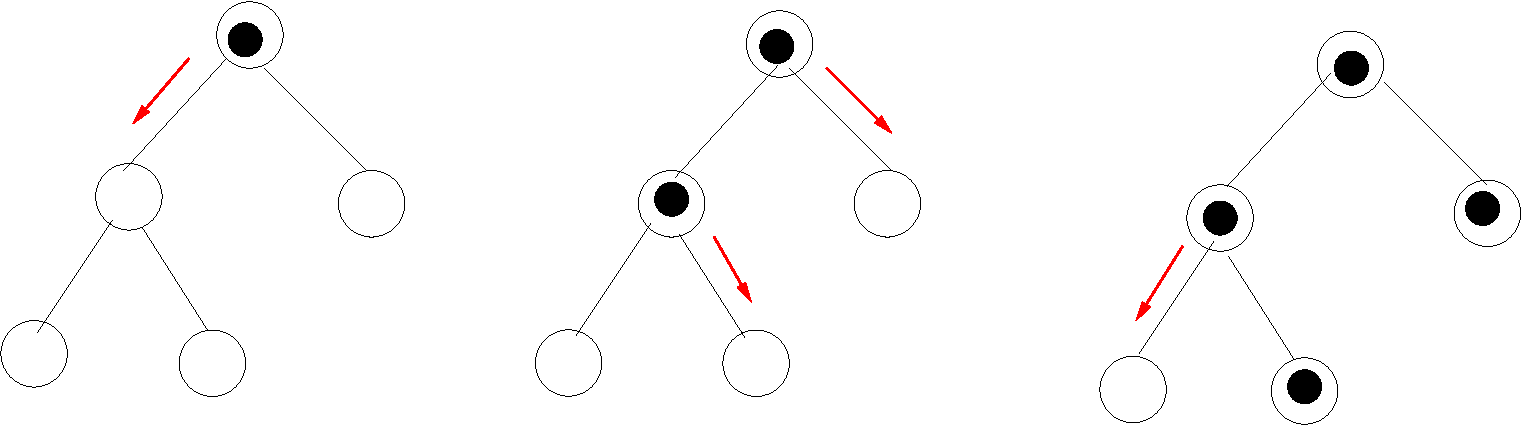
\includegraphics[scale=0.5]{tree.pdf}

Note that the order in which the messages are distributed matters. For example, in the above tree, if the root node sends the message to the right child in the first round, then
the number of rounds will be $4$.

Assume that a tree $T$ is given with nodes labeled $\{0,1, 2, \ldots, n-1\}$ and the node $0$ is the root of the tree. Further there is a two-dimensional $n \times n$ array $Child[][]$, where $k = Child[i][0]$
is the number of children of the node labeled $i$ and $Child[i][1], Child[i][2], \ldots, Child[i][k]$ denote the labels corresponding to the children of node $i$. The remaining entries in the
array are $-1$.

\begin{itemize}
\item[(a)] (4 points) Let {\sc Rounds}($i$) be a function computing the minimum number of rounds it takes to distribute the message from node $i$ to all nodes in the subtree rooted at $i$. Give a recursive formula to
compute {\sc Rounds}($i$) as a function of {\sc Rounds}($ j_1$), $\ldots$, {\sc Rounds}($j_k$), where $j_1, \ldots, j_k$ denote the children of node $i$.

{\em HINT:} What is the order in which each of the children get the message?


\ifnum\me<2
\begin{solution}

For any leaf node $i$, we have 
\begin{equation*}
 Rounds(i) = 0
\end{equation*}
For any non-leaf node $i$, let $j_{\pi_1}, \ldots, j_{\pi_k} $ be a permutation of $j_1, \ldots, j_k$ such that
\begin{align*}
& Rounds(j_{\pi_1}) \geq Rounds(j_{\pi_2}) \geq \ldots \geq  Rounds(j_{\pi_k})\\
 \implies Rounds(i) = & Max\{1+Rounds(j_{\pi_1}), 2+Rounds(j_{\pi_2}), \ldots , k+Rounds(j_{\pi_k})\}
\end{align*}

\end{solution}
\fi

\pagebreak
\item[(b)] (4 points) Write the pseudocode for the recursion with memorization dynamic programming procedure for computing  {\sc Rounds}($0$).


\ifnum\me<2
\begin{solution}

In the following psuedocode \textit{Rounds} is an array of size $n$ which holds the value of Rounds at every node in the tree and the base call is {\sc EvalRounds}(0)

\IncMargin{1em}
\begin{algorithm*}[H]
\TitleOfAlgo{{\sc EvalRounds}($i$)}
\If{Rounds(i) is not NULL}
{
	\Returnn $Rounds[i]$
}
\If{Child[i][0] is 0}{
	$Rounds[i] \leftarrow 0$\\
	\Returnn $Rounds[i]$
}

$ChildrenRounds \leftarrow$ {\sc Vector}($int$)

\For{j $\leftarrow$ 1 to n}{
	\If{Child[i][j] is not -1}{
		$Rounds[Child[i][j]] \leftarrow$ {\sc EvalRounds}($Child[i][j]$)\\
		$ChildrenRounds$.{\sc Add}($Rounds(Child[i][j])$)
	}
}

\sc{DescendingSort}($ChildrenRounds$)\\
$Rounds[i] \leftarrow -\infty$\\
\For{j $\leftarrow$ 1 to $|ChildrenRounds|$}{
	$Rounds[i] \leftarrow$ {\sc Maximum}($Rounds[i], j+  ChildrenRounds[j]$)
}
\Returnn $Rounds[i]$
\caption{Dynamic Programming Algorithm to calculate $Rounds$}
\end{algorithm*}
\end{solution}
\fi




\item[(b)] (4 points ({\bf Extra credit})) Analyze the running time of your algorithm.

\ifnum\me<2
\begin{solution}

To evaluate $Rounds(0)$, we start the base recursive call from the root node $0$ which recursively calls each of it's child and when the recursive call is returned back from it's child, store the returned value into the appropriate entry of $Rounds$ (used for memorization) corresponding to the respective child.

Each recursive call visits every node exactly once. Therefore, this takes $O(n)$ time in total. Then we sort the $Rounds$ of the node's children and then find the maximum of $j + ChildrenRounds[j]$. If every node $i$ has $k_i$ children, then the total time this step takes will be $\sum_{i=0}^{n-1}O(k_i \log k_i) + O(k_i)$ where $\sum_{i=0}^{n-1} k_i = n$

Therefore, the total time taken to evaluate $Rounds(0)$ will be $O(n) + \sum_{i=0}^{n-1}O(k_i \log k_i)$ where $\sum_{i=0}^{n-1} k_i = n$
\end{solution}
\fi

\end{itemize}


\newproblem{Max subtree}{10 points}

Given an undirected rooted tree $T$ with $n$ nodes, with possibly negative weights $w(v)$ assigned to its vertices $v$, the weight of the tree is the sum of the weights of all the nodes in the tree. (The weight of the empty tree is $0$.)

A subtree is any connected subgraph of a tree, including an empty tree as a pathological special case.
For example, in the tree below the subtrees are $\emptyset$, $\{3\}$, $\{1\}$, $\{2\}$, $\{4\}$, $\{3,1\}$, $\{3,2\}$, $\{1,4\}$, $\{3,1,4\}$, and $\{3,1,2\}$, but not $\{3,4\}$.

\vspace{1ex}
\begin{center}
%insert picture and example
\begin{tikzpicture}[level distance=1.5cm,
level 1/.style={sibling distance=3.5cm},
level 2/.style={sibling distance=1cm}]
\tikzstyle{every node}=[circle,draw]

\node (Root) {3}
    child {
    node {1}
    child { node {4} }
}
child {
    node {2}
};

\end{tikzpicture}
\end{center}

\vspace{1ex}
The goal of the problem is to design a polynomial time algorithm to find a subtree (possibly empty) with maximum weight, and analyze its running time.

\begin{itemize}
\item[(a)](4 pts) Given a node $v$, let $T(v)$ be the complete subtree of $T$ rooted at $v$ (so $T = T(T.root)$), and {\sc WithRoot}$(v)$ to be the maximum weight of a all subtrees of $T(v)$ which must include the node $v$. For example, if the tree above, {\sc WithRoot}$(1)$ is the maximum weight of sub-trees $\{1\}$ and $\{1,4\}$ (but not $\{4\}$ or the empty tree). Give the dynamic programming recurrence relation for {\sc WithRoot}$(v)$ (don't forget the base when $v$ is a leaf in $T$), and use it to analyze the running time of a dynamic-programming procedure to compute the values     {\sc WithRoot}$(v)$ for all nodes $v\in T$ (including with $T.root$).

\ifnum\me<2
\begin{solution}

This problem is similar to the problem of Maximum-Sum-SubArray. In this case, the array is replaced by a tree. Let $T$ be a tree with a root $v$ and let $v_1, \ldots, v_n$ be the children of $v$. By analogy it is easy to observe that, \textit{WithRoot(v)} is simply the union of all \textit{WithRoot($v_i$)}
 which have weight greater than 0 together with $v$

\[
WithRoot(v) = \begin{dcases*}
v & v is a leaf\\
\bigcup\limits_{\geq 0} \{WithRoot(v_i)\} \cup v & otherwise
\end{dcases*}
\]

Start from the root node $v$ and make recursive calls to each of it's child and when the recursive call is returned back, store the returned value into the appropriate entry of the array (used for memorization) corresponding to the respective node. 

A recursive call is made on every node of the tree exactly once. Therefore the time taken to calculate \textit{WithRoot(v)} for every $v \in T$ is $O(|v|)$, where $|v|$ denotes the number of nodes in the tree $T$

\end{solution}
\fi

\item[(b)](4 pts) 
Given a node $v$, let $T(v)$ be the complete subtree of $T$ rooted at $v$ (so $T = T(T.root)$), and {\sc Total}$(v)$ to be the maximum weight of a all subtrees of $T(v)$ which must may or may not include the node $v$. Assume you already solved part (a) and computed all values {\sc WithRoot}$(v)$.

Give the dynamic programming recurrence relation for {\sc Total}$(v)$ (don't forget the base when $v$ is a leaf in $T$), and use it to analyze the running time of a dynamic-programming procedure to compute the values     {\sc Total}$(v)$ for all nodes $v\in T$ (including with $T.root$, which gives the answer to the original problem). What is the running time of this algorithm?


\ifnum\me<2
\begin{solution}

Given that {\sc Total}$(v)$ may or may not include the the node $v$. We have already analyzed the case when $v$ is included. Therefore, now analyze the case when $v$ is excluded and then take the maximum of both these cases. When $v$ is excluded it will just be the maximum weight of one of it's children $v_1, \ldots, v_n$

\[
WithoutRoot(v) = \begin{dcases*}
\emptyset = 0 & v is a leaf\\
max\{Total(v_1), \ldots, Total(v_n)\} & otherwise
\end{dcases*}
\]

\begin{equation*}
Total(v) = max\{WithRoot(v), WithoutRoot(v)\}
\end{equation*}

The running time of $WithoutRoot(v)$ is similar to that of $WithRoot(v)$. A recursive call is made on every node of the tree exactly once. Hence the running time will be $O(|v|)$.

Calculating $Total(v)$ involves taking maximum of two quantities which takes $O(1)$ time. Therefore, the total running time of this algorithm is $O(|v|)$
\end{solution}
\fi

\item[(c)](2 pts)
What will the running-time of the procedures in parts (a) and (b) be if we use standard recursion, and not dynamic programming?

\ifnum\me<2
\begin{solution}

Note that the running time of part(a) is similar to that of part(b). Hence the running time of both these procedures will be effected in a similar way if we use standard recursion and not dynamic programming.

Let the total number of nodes in $T$ be $n$ and $v$ be any node in the tree then the time taken to calculate $WithRoot(v)$ and $Total(v)$ is $O(|v|)$. Let $v_1, v_2, \ldots v_n$ be the the nodes in the tree, then the total time taken without memorization is

\begin{align*}
T(n) = \sum_{i = 1}^{n} O(|v_i|)
\end{align*}

In the worst case, the tree takes the structure of a linked list. Then the above sum will evaluate to $O(n^2)$. Therefore if we use recursion without memorization, the running time increases by a factor of $n$.

However, note that in part(a) and part(b), we used memory to store the values returned by the recursive calls. Therefore, if we are allowed to use memorization in standard recursion, the running time will $O(n)$. So the running time depends on if we're allowed to use memorization or not in the standard recursion


\end{solution}
\fi

\end{itemize}

\end{document}


